%% ******************************************************
%% * This work may be distributed and/or modified under *
%% * the conditions of the LaTeX Project Public License *
%% *     http://www.latex-project.org/lppl.txt          *
%% * either version 1.3c of this license or any later   *
%% * version.                                           *
%% ******************************************************
\PassOptionsToPackage{quiet}{xeCJK}
\PassOptionsToPackage{quiet, no-math}{fontspec}
\documentclass[11pt]{article}
\usepackage{geometry,pdfpages,caption,indentfirst,setspace}
\captionsetup[table]{name={\textsc{Table}},labelsep=period}
\usepackage[level]{datetime}
\usepackage{unicode-math,xeCJK,verbatim}
\usepackage{authblk,xltxtra}
\usepackage{booktabs,diagbox,ragged2e,tabularx}
\renewcommand\tabularxcolumn[1]{>{\Centering}m{#1}}
\usepackage[toc]{multitoc}
\usepackage[mono=false]{libertine}
\linespread{1.15}
\setCJKmainfont{Chiron Sung HK}
[BoldFont=Chiron Sung HK Bold,
  ItalicFont=Kaiti SC]
\usepackage{hyperref,cprotect,xcolor,verbatim,tikz}

\definecolor{pkgcolor}{Hsb}{103,.8,.5}
\definecolor{moducolor}{Hsb}{290,.8,.5}
\definecolor{cmdcolor}{Hsb}{188,.8,.5}
\definecolor{filecolor}{Hsb}{207,.6,.7}
\definecolor{H1}{Hsb}{349,.8,.8} % 海棠紅 (Hangzhou MTR L 1 )
\definecolor{H2}{Hsb}{23, .8,.8} % 丹桂橙 (Hangzhou Metro 2 )
\definecolor{H3}{Hsb}{48, .8,.8} % 柠檬黄 (Hangzhou Metro 3 )
\definecolor{H4}{Hsb}{103,.8,.8} % 香樟绿 (Hangzhou Metro 4 )
\definecolor{H5}{Hsb}{188,.8,.8} % 青藍色 (Hangzhou MTR L 5 )
\definecolor{H6}{Hsb}{207,.8,.8} % 海洋蓝 (Hangzhou Metro 6 )
\definecolor{H7}{Hsb}{290,.8,.8} % 浪漫紫 (Hangzhou Metro 7 )
\hypersetup{colorlinks,urlcolor=H6,linkcolor=H2,filecolor=filecolor,pdfstartview=FitH,pdfview=FitH,pdfcreator=XeTeX output}

\def\pkg#1{\texorpdfstring{\textcolor{pkgcolor}{\textsf{#1}}}{“#1”}}
\def\mode#1{\texorpdfstring{\textcolor{moducolor}{\textsf{#1}}}{“#1”}}
\def\cmd#1{\texorpdfstring{\textcolor{cmdcolor}{\textsf{#1}}}{“#1”}}
\def\datechange#1#2{%
  \noindent{\makebox[\textwidth][r]{\color{H7}\rule{1.15\textwidth}{.4pt}}}
  \noindent\makebox[0pt][r]{\makebox[-3em][r]{\small\textbf{\textcolor{H7}{#1}}}\;\;}{\sffamily Update: \ignorespaces#2}}
\makeatother

\title{\bfseries\pkg{LiteTable} -- 多彩的课程表\textsf{\LaTeX} 模板}
\author{\href{https://www.hdu.edu.cn}{杭州电子科技大学}, 夏明宇}
\yyyymmdddate
\date{\today}
\affil{\href{mailto:xiamyphys@gmail.com}{\texttt{xiamyphys@gmail.com}}}
\date{\today\quad Version 2.4a\thanks{%
  \url{https://github.com/xiamyphys/litetable}}}
\begin{document}
\maketitle

\vspace{-2em}
\begin{abstract}
\pkg{LiteTable} 模板提供了一个多彩的课程表设计,本文档为 \pkg{LiteTable} 模板的说明文档.
\end{abstract}

\tableofcontents

\clearpage

\section{Introduction}

\subsection{本模板的目的}
本模板提供了一个多彩的课程表设计. 

如果你在使用本模板时遇到问题,或者有更好的建议,或者你想参与本模板或本人其他模板的开发,欢迎通过邮件 \href{mailto:xiamyphys@gmail.com}{xiamyphys@gmail.com} 联络我.

同样,你也可以加入我的\textsf\LaTeX{} 技術交流群 \href{https://qm.qq.com/q/OnHzbNvVAG}{QQ Group: 760570712} 与我交流,来获取模板的内测版本.

\subsection{所需宏集}
本模板基于 \pkg{standalone} 文档类开发. 其需要 \pkg{tikz} 宏集去绘制图形,\pkg{kvoptions} 和 \pkg{etoolbox} 宏集用于提供全局模式,\pkg{expl3} 宏集用于支持数组,\pkg{ctex}宏集用于支持中文语言,\pkg{fontawesome5} 宏集提供一系列精美的图标.

\subsection{安装并载入 \pkg{LiteTable} 模板}
免安装使用方法如下,从 \href{https://github.com/xiamyphys/LiteTable}{GitHub} 或 \href{https://ctan.org/pkg/litetable}{CTAN} 下载最新的 \verb|litetable.cls| 文件并将它保存至你的项目根目录. 这种安装方式是最便捷的,但是当模板更新后,你需要手动替换 \verb|.cls| 文件.

然而我强烈建议您使用终端机去执行以下命令,以将所有宏集更新到最新版本,并安装此模板
\begin{verbatim}
    sudo tlmgr update --self
    sudo tlmgr update --all
\end{verbatim}

如果您所在的地区存在网路封锁(如 GFW 干扰),你可以选择合适的镜像网站或其他方法\footnote{请遵守当地的网路条例.}. 欲详细了解,请前往 \href{https://tex.stackexchange.com/questions/55437/how-do-i-update-my-tex-distribution}{How do I update my TEX distribution?}

本模板提供了三个选项:\mode{style},\mode{direction} 和 \mode{font}. 只需将你要使用的选项模式分别添加在你的 \verb|.tex| 文件中命令 \verb|\documentclass[ ]{litetable}| 的方括号中即可.

\subsection{兼容性}
所使用的测试环境为 macOS + MacTeX 2023 / Overleaf,都可在 \XeLaTeX{} 编译方式下顺利运行, Windows, Linux 和 Unix 平台兼容性未知.

\section{\pkg{LiteTable} 的全局选项}
\begin{verbatim}
  \documentclass[options]{litetable}
\end{verbatim}

\subsection{\mode{style} 选项}
此选项有两个模式,\mode{round} 和 \mode{sharp},可分别使课程块圆角或直角显示,默认为直角.

\subsection{\mode{direction} 选项}
此选项有两个模式,\mode{portrait} 和 \mode{landscape}, 可分别使课程表以纵向或横向显示.

\subsection{\mode{font} 选项}
此选项有两个模式,\mode{times} 和 \mode{libertinus},可分别使字体为 ``Times New Roman'' 或 ``Libertinus'',默认为 ``Times New Roman''\footnote{在使用 ``Libertinus'' 模式前请确保电脑中已安装该字体.}.

\section{\pkg{LiteTable} 的命令}

\subsection{\cmd{makeframe} 命令}
\begin{verbatim}
  \makeframe{Timetable -- Semester 5}
\end{verbatim}

此命令可建立一个标题为 ``Timetable -- Semester 5'' 的空白课程表.

\subsection{\cmd{weeklist} 命令}
\begin{verbatim}
  \weeklist{
    \bfseries\textcolor{W1}{\faIcon{moon}~星期一},
    \bfseries\textcolor{W2}{\faIcon{fire}~星期二},
    \bfseries\textcolor{W3}{\faIcon{water}~星期三},
    \bfseries\textcolor{W4}{\faIcon{tree}~星期四},
    \bfseries\textcolor{W5}{\faIcon{coins}~星期六}
  }
\end{verbatim}

此命令可在课程表顶部添加工作日,你可以自由决定工作日的显示样式,如名称,颜色甚至是前面的 logo\footnote{由 \pkg{fontawesome5} 宏集支持.}.

课程表可根据你输入的时间组数自动生成相应的列数. 如上方代码共有 5 个工作日,就会生成 5 列的课程表.

\subsection{\cmd{timelist} \cmd{classnum} 命令}
\begin{verbatim}
  \timelist{
    8:05,8:55,10:00,10:50,11:40,13:30,14:20,15:15,16:05,18:30,19:20,20:10;
    8:50,9:40,10:45,11:35,12:25,14:15,15:05,16:00,16:50,19:15,20:05,20:55
  }

  \classnum{14}
\end{verbatim}

命令 \cmd{timelist} 可将时间添加至课程表的左侧,内容的第一行是每节课程开始时间,第二行是每节课程的结束时间,时间之间用逗号(\verb|,|)分隔,第一行与第二行之间用分号(\verb|;|)分隔.

课程表可根据你输入的时间组数自动生成相应的行数. 如上方代码共有 12 组时间,就会生成 12 行的课程表.

命令 \cmd{classnum} 可直接指定课程表上你想要生成的行数并不会在课程表左侧添加时间,左侧只会有一列\emph{在每行竖直居中}的序号.

下面的表格整理了两个命令不同使用情况下的不同效果.
\begin{table}[!ht]
\centering
\caption{命令 \cmd{timelist} and \cmd{classnum} 的使用情况.}

\begin{tabularx}{\textwidth}{c >{\raggedright\arraybackslash}X >{\raggedright\arraybackslash}X}
  \toprule
  \diagbox{\cmd{classnum}}{\cmd{timelist}} & \multicolumn{1}{c}{使用} & \multicolumn{1}{c}{不使用}\\
  \midrule
  使用   &
  效果和命令 \cmd{timelist} 描述相同\newline 但生成行数由 \cmd{classnum} 决定 &
  效果和命令 \cmd{classnum} 描述相同\\
  \midrule
  不使用 &
  效果和命令 \cmd{timelist} 描述相同          &
  效果和命令 \cmd{timelist} 描述相同\newline\emph{并默认生成 12 行}.\\
  \bottomrule
\end{tabularx}
\end{table}

\begin{itemize}
  \item 若命令 \cmd{timelist} 中有 12 组时间,命令 \cmd{classnum} 传递的数值为 14,那么课程表的左侧会只有 1 -- 12 行有时间标注,最后两行没有时间标注但最后两行的标号仍然偏上方,并不会竖直对齐.
  \item 若命令 \cmd{timelist} 中有 14 组时间,命令 \cmd{classnum} 传递的数值为 12,那么只会生成 12 行的课程表并且左侧均有时间标注,也就是在命令 \cmd{timelist} 中输入的最后两组时间无效.
\end{itemize}

\subsection{\cmd{weeks} 命令}
\begin{verbatim}
  \weeks{Week 1 -- 16}
\end{verbatim}

此命令可指定命令 \cmd{course} 第 7 个参数的默认值.

\subsection{\cmd{course} 命令}
\begin{verbatim}
  \course[H1]{8}{9}{群论}{第6教研楼 · 中211}{Li Ge}[Week 1 -- 16]
\end{verbatim}

此命令共有7个参数.
\begin{itemize}
  \item 第 1 个为课程块的颜色,从 ``H1'' 到 ``H9'' 供选择,此参数是可选参数,默认为 ``H1''.
  \item 第 2 个和第 3 个为课程的起始节数和结束节数.
  \item 第 4, 5, 6 个分别为课程的名称,地址和教师的名字.
  \item 第 7 个为课程的首末周,此参数是可选参数,默认值由命令 \cmd{weeks} 指定,若未指定则默认值为 ``Week 1 -- 12''.
\end{itemize}



\subsection{\cmd{newday} 命令}
此命令可切换当前日到第二天,此时课程块会右移一格.

\subsection{\cmd{more} 命令}
\begin{verbatim}
  \more{ · School Start: 04 / 03 / 2024  · Summer Vacation: 05 / 07 / 2024}
\end{verbatim}
此命令可在课程表末尾添加备注信息.

\subsection{\cmd{sticker} 命令}
\begin{verbatim}
  \sticker{favicon}
\end{verbatim}
在使用此命令后页面的右下方会添加一张贴纸.

\subsection{\cmd{(re)rotatepage} 命令}
\cmd{rotatepage}命令可临时更改课程表的方向,\cmd{rerotatepage} 命令可恢复课程表原来的方向.

\section{已知问题:分辨率溢出}
\begin{verbatim}
  Dimension too large. <recently read> \pgfmath@x
\end{verbatim}

当启用 \mode{landscape} 模式并添加 7 个及以上的工作日 (?虽然 `添加7 个以上工作日' 一般碳基生物做不出来这种事),便会给出该报错.

这主要是因为 \emph{\textsf{\TeX} 没有内置的浮点数表示} (Reference: \cprotect{\href{https://tex.stackexchange.com/a/545416/299948}}{How to solve the error `Dimension too large. <recently read> \verb|\pgfmath@x|' while doing the calculations in the table}).

如果你能通过优化算法或其他方式解决该问题,欢迎通过 GitHub: \url{https://github.com/xiamyphys/litetable} 提交你的代码,或通过邮件 \href{mail:xiamyphys@gmail.com}{\ttfamily xiamyphys@gmail.com} 联络我.

\section{版本历史}

课程表的设计源于\href{https://www.hdu.edu.cn}{杭州电子科技大学}杭电助手学生课表页面(仅本校师生可访问). 页面排版十分精美,于是本人使用 \textsf{\LaTeX{}} 复刻出了课程表样式,并制作成模板分享给大家.

\textsf{\bfseries Version 1.0} 于01/09/2023完成开发,并发布在 \href{https://www.latexstudio.net/index/details/index/mid/3625.html}{\textsf{\LaTeX}工作室} (杭州萧山)和\href{http://xhslink.com/od7Ycw}{小红书}上,赢得了许多人的喜爱.

\textsf{\bfseries Version 2.0a}于01/11/2023完成开发,并发布在 \href{https://www.latexstudio.net/index/details/index/mid/3636.html}{\textsf{\LaTeX}工作室} (杭州萧山)和\href{http://xhslink.com/od7Ycw}{小红书}上. 此版本使用 \verb|.cls| 文件,使 \verb|main.tex| 文件更简洁. 同时,此版本添加了全局模式,可设置 ``课程块'' 显示为圆角或直角. 此版本也支持一个 \verb|.tex| 文件中生成多张课表.

\textsf{\bfseries Version 2.1a} 于05/11/2023完成开发. 支持 libertinus 字体.

\textsf{\bfseries Version 2.2a} 于31/01/2024完成开发. 此版本修复了分辨率超出的 bug,更改纸张类型为美国信纸并支持自定义课程起始和结束时间.

\textsf{\bfseries Version 2.3a} 于02/02/2024完成开发. 此版本支持根据所输入的时间组数自动生成相应的行数,并支持课程表以纵向或横向显示.

\textsf{\bfseries Version 2.3b} 于03/02/2024完成开发. 此版本优化坐标计算,提升编译速度.

\textsf{\bfseries Version 2.4a} 于24/02/2024完成开发. 元宵节快乐! 此版本支持自定义工作日显示样式,支持隐藏时间并仅显示竖直对齐课程序号,支持设置默认首末周.

\clearpage

\datechange{01/09/2023}{Version 2.0a}
\begin{itemize}
    \item 支持课程块显示为圆角或直角.
    \item 支持一个 \verb|.tex| 文件中生成多张课表.
\end{itemize}

\datechange{05/11/2023}{Version 2.1a}
\begin{itemize}
    \item 支持 libertinus 字体.
\end{itemize}

\datechange{31/01/2024}{Version 2.2a}
\begin{itemize}
    \item 修复了分辨率超出的 bug.
    \item 更改纸张类型为美国信纸.
    \item 支持自定义课程起始和结束时间.
    \item 支持在页面右下角添加一个你喜欢的小贴纸.
    \item 提供简体中文说明文档.
\end{itemize}
\setstretch{1}
\datechange{2024/02/02}{Version 2.3a}
\begin{itemize}
  \item 支持根据所输入的时间组数自动生成相应的行数.
  \item 课程表可纵向或横向显示.
\end{itemize}

\datechange{2024/02/03}{Version 2.3b}
\begin{itemize}
  \item 优化坐标计算,提升编译速度.
\end{itemize}

\datechange{\today}{Version 2.4a}
\begin{itemize}
  \item 支持自定义工作日显示样式.
  \item 支持隐藏时间,仅显示竖直对齐课程序号.
  \item 支持设置默认首末周.
\end{itemize}

\appendix

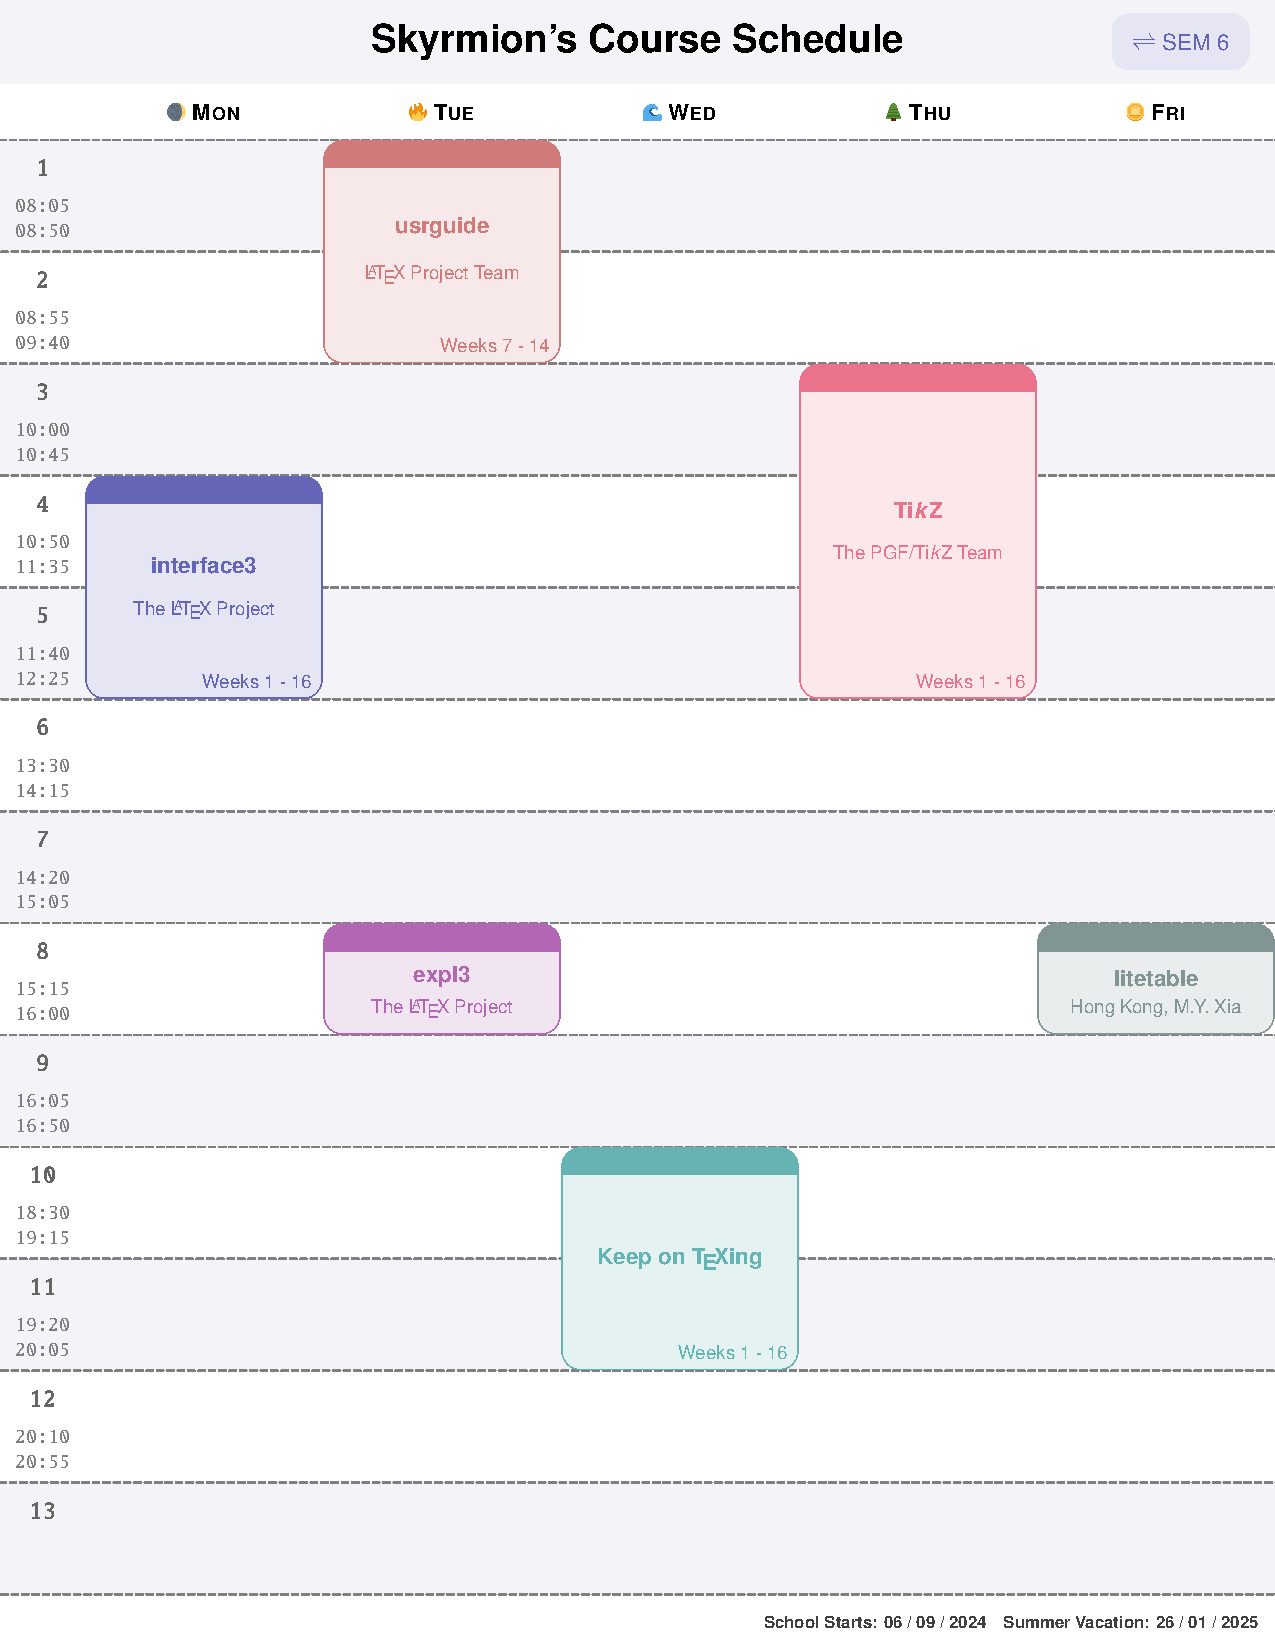
\includepdf[pages={1,3}]{litetable-demo.pdf}
\includepdf[pages={2,4},nup=1x2,pagecommand={
  \tikz[remember picture, overlay]
  \node [rotate=90,below,yshift=-1em] at (current page.west) {\bfseries\LARGE Document Example: \texttt{litetable-demo.tex}};
  }
]{litetable-demo.pdf}

\end{document}